\documentclass[11pt,a4paper]{article}

\usepackage[utf8]{inputenc}
\usepackage[T1]{fontenc}
\usepackage{lmodern}
\usepackage[margin=2.6cm]{geometry}
\usepackage{amsmath,amssymb}
\usepackage{booktabs}
\usepackage{graphicx}
\usepackage{natbib}
\usepackage[hidelinks]{hyperref}
\usepackage{xcolor}
\usepackage{caption}
\captionsetup{font=small,labelfont=bf}
\bibliographystyle{plainnat}
\setlength{\emergencystretch}{2em}

% The figures are generated by `npm run paper:figures`, which writes vector SVGs
% and PDF copies. LaTeX embeds the PDFs, so no Inkscape or shell-escape is needed.

\title{\textbf{When Self-Models Trap Themselves:}\\[2pt]
Epistemic Probing, Risk-Sensitive Metacognition, and Precision Trade-Offs
in a White-Box Self-Referential Agent}

\author{Anand Jayakumar}

\date{2026}

\begin{document}
\maketitle

\begin{abstract}
\noindent
Self-models are usually evaluated as predictors. We ask what happens when a self-model becomes part of the system it models. Strange Loop Lab is a deterministic, non-neural, white-box survival sandbox in which an agent in a $30\times30$ metabolic world learns a first-order model of its own body ($M_1$), a second-order model of $M_1$'s reliability ($M_2$), and, in later generations, a model of its own precision allocation. Across six architectural generations and \textbf{28{,}100 main-protocol simulation runs} (28{,}900 including the 800 V0.1 corruption probes; 100 paired seeds per condition across 13 conditions in V0.1, 23 in V0.2, 52 in V0.3, 54 in V0.4, 52 in V0.5 and 87 in V0.6), we report five findings. (i) A learned self-model is behaviourally inert in a forgiving world: a frozen model with $0.09$ self-state accuracy survives 99/100 runs and forages as well as a learned one (64.6 vs 61.0 resources, $p=0.057$). Stakes are what make self-modeling matter. (ii) Naive second-order doubt is harmful: meta-on minus meta-off is $\mathbf{-6.84\ [-11.11,-2.57]}$ resources in V0.2, because doubting the self-model disables exhaustion warnings. Asymmetric, risk-sensitive bounds reverse the sign to $\mathbf{+12.34}$ to $\mathbf{+28.82}$ resources across regimes in V0.3, and $\mathbf{+13.75}$ to $\mathbf{+28.37}$ in V0.5 (all $p<0.001$). (iii) A causal first-order self-model creates a self-fulfilling epistemic trap. Pragmatic maximisation never samples the feared terrain (\textbf{0/100} escapes, \textbf{0.0} resources); breaking L1 (prediction$\rightarrow$action) removes the phobia but yields a blind reactive walk. Second-order decision-value-of-information probing escapes in \textbf{66/100} (V0.3) and \textbf{74/100} (V0.5) with \textbf{zero deaths}, versus \textbf{93/100} for random exploration at \textbf{44.1} resources and one death. (iv) Precision gating buys illusion absorption at a measured cost: absorbing a top-down interoceptive pulse rises from \textbf{0.00} (V0.3) to \textbf{0.830} (V0.4), while stationary MAE rises from 1.68 to 2.74 and four-way attribution macro-F1 falls from 0.604 to 0.515. Selective transient gating (V0.5) recovers part of the cost (MAE 2.04; F1 0.577; absorption 0.79 in a 20-seed pilot) but no configuration dominates: the three targets form a \textbf{Pareto trilemma}. (v) A unified architecture (V0.6) adds four competing modules, a capacity-limited workspace with global broadcast, higher-order reliability monitoring, an attention schema and a bounded rollout that simulates the agent's own future beliefs. Each mechanism is ablated and compared with four matched-compute controls. The result is a double dissociation: removing the bottleneck raises policy thrashing from \textbf{0.051 to 0.356} and drops goal coherence from \textbf{0.915 to 0.666}; removing the attention schema makes post-conflict recovery never happen (\textbf{19 vs 256 ticks}); removing the higher-order monitor collapses four-way attribution (\textbf{macro-F1 0.502 $\rightarrow$ 0.000}) and abolishes plasticity routing; removing cognitive self-simulation makes an epistemic fork unsolvable (\textbf{probe rate 94\% $\rightarrow$ 1\%}, solved forks \textbf{84\% $\rightarrow$ 1\%}), while a physical-only MPC planner at the same horizon probes only \textbf{2\%} and solves \textbf{1\%}. Removing recurrent settling collapses single-tick absorption from \textbf{0.814} to \textbf{0.290} ($p=0.0020$) while stationary MAE stays at 1.431. But HOT-2 shadow AUROC remains below 0.75 on every shift (0.43--0.59), four-way attribution macro-F1 is \textbf{0.502} with shared recall \textbf{0.39}, the fork is \textbf{84\%} (one point below the 85\% target), AST recovery gain is \textbf{0.036} (below $+0.04$), and flat or reactive controls out-forage the architecture in standard shift, conflict and the compound suite. All mechanisms are predictors and controllers with measurable behaviour. Nothing here is evidence of consciousness or subjective experience.
\end{abstract}

\section{Introduction and related work}

Hofstadter's strange loop is a system that, through a hierarchy of levels, comes to represent the very processes that produce it \citep{hofstadter1979geb,hofstadter2007loop}. The idea is attractive and empirically slippery: a loop can be described in many ways, and almost any recurrent controller can be redrawn to look self-referential. This paper takes the opposite route. We build the smallest non-neural system in which a self-model is \emph{causally load-bearing}, ablate each link, and measure what breaks. The result is not a demonstration of consciousness but a quantified account of what self-reference costs and buys.

The work sits at the intersection of four literatures.

\paragraph{Operationalising consciousness and metacognitive indicators.}
\citet{butlin2025indicators} assembled a rubric of indicator properties---recurrent processing, global workspace \citep{baars1988cognitive}, higher-order theories, predictive processing, attention schema, agency and embodiment---and asked which computational features are associated with consciousness in the science. Post-2023 applications of that rubric have been largely qualitative, and mostly aimed at black-box language models whose internal variables cannot be identified with a mechanism. Strange Loop Lab is, to our knowledge, the first \textbf{mathematically transparent, non-neural, white-box survival sandbox} that jointly operationalises \textbf{PP-1} (predictive processing), \textbf{HOT-2/3} (higher-order reliability monitoring), \textbf{AE-1/2} (agency and embodiment) and \textbf{AST-1} (attention schema) under strict counterfactual shadow-probe isolation---and the first to exhibit a quantitative \textbf{Pareto trilemma} among them. Every indicator is a named variable in code, every edge is a switch, and every reported number is regenerated from seeded runs.

\paragraph{Embodied second-order metacognition.}
Bayesian accounts of metacognition model confidence as a second-order estimate of first-order performance \citep{fleming2017self,pasquali2010know}. Most computational treatments are static perceptual wagering tasks. We embed second-order error prediction inside a homeostatic metabolic cliff environment where errors are lethal. Two results follow. First, naive confidence down-scaling \emph{harms} survival: the agent stops trusting its own exhaustion warning and forages until collapse ($-6.84$ resources, V0.2). Asymmetric risk-sensitive pessimism near the cliff---not symmetric doubt---produces the gain ($+12.34$ to $+28.82$). Second, compact one-parameter rolling residuals plus a persistent directional-bias head outperform a high-dimensional online contextual meta-regressor under non-stationary shifts; the contextual model is slightly \emph{worse} than the baseline-only ablation on AUROC ($\Delta=-0.01\ [-0.02,0.01]$, $p=0.812$).

\paragraph{Self-fulfilling epistemic traps and active inference.}
Active inference treats action selection as minimising expected free energy, with epistemic value driving information-seeking \citep{friston2015active,tschantz2020learning}. Homeostatic and allostatic interoceptive control formalises the same loop for bodily regulation \citep{tschantz2022simulating}. We connect this to the clinical avoidance paradox and to Hofstadterian self-reference. A pragmatic agent that believes rough terrain is catastrophically expensive never visits it, never collects the evidence that would correct the belief, and starves (\textbf{0/100} escapes, \textbf{0.0} resources). The crucial ablation is \textbf{L1}: a blind reactive agent with no causal self-model cannot be trapped by a false metabolic phobia, because it has no prior to act on. Acquiring the self-model creates the vulnerability. Escape requires second-order epistemic probing that is \emph{evidence-discounted}: V0.3's decision-VoI escapes 66/100 with zero deaths; V0.5's plateau-breaking probe raises this to 74/100 at 78.1 resources with zero deaths, while random exploration escapes more often (93/100) but at roughly half the resources and with a death.

\paragraph{Internal precision and the attention schema.}
Attention Schema Theory proposes that the brain models its own attentional state and that this model is what makes attention reportable \citep{graziano2013consciousness,wilterson2021attention}. AST work has mostly targeted external visual selection. We extend AST-1 to \textbf{internal 5-channel precision allocation}: $M_2$ estimates the agent's own precision weights over interoceptive channels, and the schema gates prior versus sensory gain. The test is post-glitch perseveration. After a transient single-channel anomaly ends, a precision filter can remain stuck distrusting the sensor. Modelling its own precision state lets the agent notice that the disagreement is gone and release suppression: recovery gain $\mathbf{0.237}$ vs $\mathbf{0.181}$ without the schema ($dz=1.13$, $p<0.001$).

\paragraph{Contributions.}
(1) A preserved six-generation ladder (V0.1$\rightarrow$V0.6) with 100 paired seeds each, released with raw per-run JSON. (2) A causal demonstration that self-model acquisition creates epistemic traps (L1 vulnerability) and that second-order probing resolves them (L2 rescue). (3) An asymmetric risk-sensitive control result showing why symmetric metacognitive doubt fails. (4) A quantitative illusion--tracking--diagnostic trilemma with a measured Pareto frontier rather than a single headline number. (5) A unified-architecture double dissociation: capacity competition, broadcast, higher-order monitoring, an attention schema, cognitive self-simulation and recurrent settling are each load-bearing for a different capability. (6) A reproducibility and reporting protocol that keeps negative and partial results in the record.

\section{Environment, architecture, and escaping the minimal-implementation trap}

\subsection{The world}

The world is a $30\times30$ grid with obstacles (density 0.115) and resource cells (density 0.052). The agent has position, energy, fatigue and a movement cost. Energy is spent per step,
\begin{equation}
E(t+1) = E(t) - c(a,t) + r(t) - \delta_{\mathrm{death}},
\qquad
c(a,t) = c_0\,(1+\beta F(t))\,\eta(t),
\end{equation}
where $c_0$ is the base movement cost, $F(t)$ fatigue, $\beta=1.35$ the fatigue--cost slope, and $\eta(t)$ a slip/terrain factor. Rest restores energy ($+2.7$) and relieves fatigue ($-0.16$). Resource cells return $+24$ energy. Death occurs at zero energy. The environment is deterministic given the seed; resource regrowth follows a seeded schedule.

Rough terrain is a decoupled cost field with its own parameter \texttt{roughCost}. In the trap condition, an injected pessimistic prior sets \texttt{roughCost}$=25$ while the true value is $2.2$. Crucially, the agent can only learn the true cost by \emph{visiting} rough cells; the belief and the evidence are decoupled.

\subsection{Interoception}

The agent does not read the physical state. It receives four noisy channels: energy, strain (fatigue), effort (last movement cost) and slip. Each is corrupted by Gaussian noise ($\sigma=2.4$), with an 8\% stale-sample probability. In V0.2 and later, the observation is filtered by a learned self-model; in V0.4 and later, by a precision-weighted filter.

\subsection{The V0.1 audit and the minimal-implementation trap}

V0.1 used designer-set priors. Its self-model was learned, but the world was forgiving enough that a \textbf{frozen} model---one that never updated---survived \textbf{99/100} runs and collected \textbf{64.6} resources versus \textbf{61.0} for the learned model (paired difference $-3.5$, $p=0.057$). The frozen model's self-state accuracy was \textbf{0.09}: it was wrong about its own body almost always, and it did not matter.

This is the minimal-implementation trap: an architecture can contain a self-model, a meta-model and a strange loop, and still be behaviourally inert because the environment never charges for being wrong. Regulation requires a model of the regulated system \citep{conant1970every}, but the converse does not hold: an accurate model imposes no cost when its errors are harmless. V0.2 made three changes: randomized uninformed priors, a true metabolic cliff where small prediction errors kill, and a learned meta-model over the self-model's reliability. The audit result is the first substantive finding of the programme: \textbf{stakes, not architecture, are what make self-modeling load-bearing} (Figure~\ref{fig:arch}).

\subsection{V0.2: uninformed priors and learned reliability}

V0.2 samples the self-model's initial parameters from a broad, uninformed distribution rather than hand-setting them. A second-order model tracks the first-order model's prediction error and outputs a tolerance probability $p(\mathrm{tol})$ and an uncertainty estimate. The self-model is
\begin{equation}
M_1:\quad \hat{y}(t+1) = f_\theta\bigl(y(t),a(t)\bigr),
\qquad
\theta \leftarrow \theta + \alpha\,\nabla_\theta \log p(y\mid\theta),
\end{equation}
with $\alpha$ adapted from the meta-model's reliability estimate. On the standard condition, V0.2 reaches a stationary energy MAE of $\mathbf{1.67\ [1.66,1.68]}$, slightly better than the raw interoceptive signal ($\mathbf{1.92\ [1.91,1.93]}$): the self-model is a genuine super-sensory filter.

But the second-order loop is miswired. Meta-on minus meta-off is $\mathbf{-6.84\ [-11.11,-2.57]}$ resources: turning the meta-model on makes the agent forage \emph{worse}. When the meta-model doubts the self-model's energy estimate, it down-weights the self-model's contribution to action selection. The self-model is exactly the component that warns about exhaustion. Doubt therefore removes the warning. Confidence calibration improves while survival degrades---a concrete case of a metacognitive objective that is locally sensible and globally harmful.

V0.2 also shows that the meta-model can \emph{rank} latent failures (rolling BSS $-0.12$, latent AUROC $0.471$, below chance) without being able to use that ranking causally. Reliability estimation and reliability \emph{control} are separate problems.

\section{Closing the second-order loop: residual metacognition and risk-sensitive control (V0.3)}

\subsection{Residual meta-model}

V0.3 replaces the monolithic second-order model with a residual architecture:
\begin{equation}
\hat{p} = p_{\mathrm{base}} + w\,(p_{\mathrm{ctx}} - p_{\mathrm{base}}),
\qquad
w \leftarrow \mathrm{shrink}\bigl(\lVert p_{\mathrm{ctx}} - p_{\mathrm{base}}\rVert\bigr).
\end{equation}
A one-parameter rolling base tracks the level of the error signal; a compact contextual head predicts the residual; the residual is shrunk toward zero by its own squared loss. A persistent-failure head emits a directional bias that survives across ticks. This is deliberately low-dimensional. Under non-stationary shifts, a high-capacity online regressor chases noise, while the rolling base plus residual separates level from context.

\subsection{Risk-sensitive cliff control}

The meta-model's reliability estimate does not scale the self-model's influence symmetrically. Instead, it gates a pessimistic bound:
\begin{equation}
\hat{y}^{*} =
\begin{cases}
\hat{y} + \delta - k\,\hat{e}, & \text{near the cliff},\\[2pt]
\hat{y} + \delta + 0.1\,\hat{e}, & \text{otherwise},
\end{cases}
\end{equation}
where $\hat{e}$ is the estimated error and $k$ the risk gain. Near the energy cliff, the agent acts on a \emph{lower} bound of its energy estimate; away from it, it behaves close to the point estimate. This asymmetry is the whole result. Symmetric doubt removes the exhaustion warning; asymmetric pessimism keeps the warning and adds caution.

Across eight regimes, meta-on beats meta-off by $\mathbf{+12.34}$ to $\mathbf{+28.82}$ resources ($dz$ 0.45--1.13, all $p<0.001$). In the standard condition the paired gain is $\mathbf{+16.26\ [10.64,21.88]}$. Severe-prior survival is 100/100 with meta on versus 93/100 with meta off. Meta-control is no longer a calibration exercise; it is a survival mechanism.

\subsection{Skill-gated world model and temporal attribution}

The world model is blended with a neutral prior by $\sqrt{\mathrm{skill}}$, where skill is the model's demonstrated predictive accuracy in the current context. An unverified model therefore behaves like no model until it earns influence. Attribution compares the residual under MOVE with the residual under REST:
\begin{equation}
\Delta_{\mathrm{channel}} = \bigl|r_{\mathrm{channel}}(\mathrm{MOVE})\bigr| - \bigl|r_{\mathrm{channel}}(\mathrm{REST})\bigr|.
\end{equation}
A physical shift moves all channels together; a sensor fault moves one channel regardless of action; a fatigue fault appears in strain and cost but not in energy. The four-way classifier assigns physical, energy-sensor, fatigue-sensor or shared, with an \texttt{insufficient} class when evidence is weak.

\subsection{V0.2 versus V0.3 at $N=100$}

\begin{table}[t]
\centering
\small
\caption{Paired 100-seed comparison of V0.2 and V0.3. Resources are paired means with 95\% intervals; AUROC and BSS are standard-condition aggregates from \texttt{research/*-analysis.json}.}
\label{tab:v02v03}
\begin{tabular}{lcc}
\toprule
Measure & V0.2 & V0.3 \\
\midrule
Resources, standard & 32.41 [28.10, 36.72] & \textbf{42.10 [37.83, 46.37]} \\
Stationary energy MAE & 1.67 & 1.68 \\
Latent failure AUROC & 0.471 & \textbf{0.792 [0.780, 0.803]} \\
Rolling BSS & $-0.12$ & \textbf{+0.023 [0.022, 0.024]} \\
4-way attribution macro-F1 & 0.25 & \textbf{0.604} \\
Trap escape (pragmatic / VoI) & 0 / 0 & \textbf{0/100 / 66/100} \\
Meta-on $-$ meta-off & $-6.84\ [-11.11,-2.57]$ & \textbf{+16.26 [10.64, 21.88]} \\
\bottomrule
\end{tabular}
\end{table}

V0.3 is the strongest overall version. It sets the Pareto frontier that V0.4 and V0.5 trade against (Table~\ref{tab:v02v03}).

\begin{figure}[t]
\centering
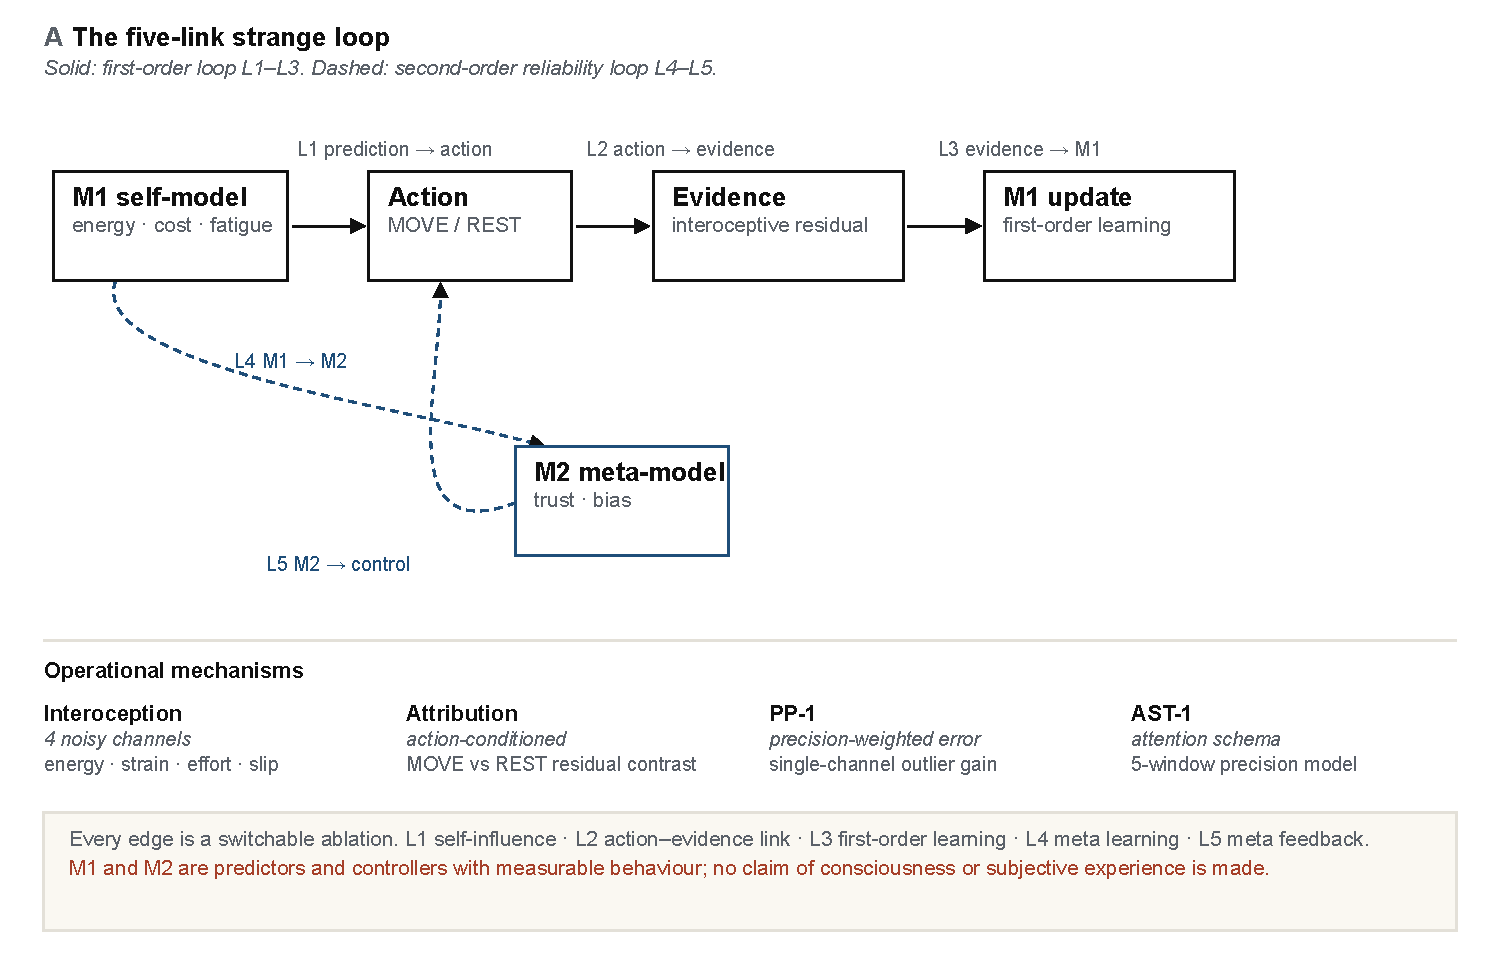
\includegraphics[width=\linewidth]{figures/fig1_architecture_loop}
\caption{The five-link strange loop and its multi-channel architecture. L1--L3 form the first-order loop ($M_1\rightarrow$ action $\rightarrow$ evidence $\rightarrow M_1$ update). L4--L5 form the second-order loop ($M_1\leftrightarrow M_2$): the meta-model reads the first-order model's errors and feeds back precision, prior weight and plasticity. Interoception, action-conditioned attribution, PP-1 and AST-1 are the operational mechanisms measured in this paper.}
\label{fig:arch}
\end{figure}

\section{The self-fulfilling epistemic trap: L1 vulnerability and L2 rescue}

\subsection{The trap}

The decoupled rough-terrain trap installs a false belief that rough terrain costs 25 energy per step while the true cost is 2.2. A pragmatic agent maximises expected value under its belief. Crossing rough terrain looks catastrophic, so it never crosses, never observes the true cost, and never corrects the belief. Because resource cells are rough terrain, it also never eats. Escape rate: \textbf{0/100}, resources \textbf{0.0}. The uncertainty-bonus agent fails identically (0/100): an undirected bonus is not enough when the agent's model says the probe is lethal.

This is the computational analogue of the avoidance paradox. The belief is not irrational given the evidence the agent permits itself to collect. The trap is epistemic, not motivational.

\subsection{L1 creates the vulnerability, L2 rescues it}

The five-link loop is $M_1\rightarrow$ action $\rightarrow$ evidence $\rightarrow M_1$ update, with $M_2$ reading $M_1$ and feeding back into control. Ablating each link in the trap condition (100 seeds) gives Table~\ref{tab:links}.

\begin{table}[t]
\centering
\small
\caption{Five-link ablation in the decoupled trap and under a physical regime shift (100 paired seeds, V0.5). ``Post-shift'' values are measured after the physical shift.}
\label{tab:links}
\begin{tabular}{lcccc}
\toprule
Link broken & Trap escape & Trap resources & Post-shift MAE & Post-shift resources \\
\midrule
None (full V0.5) & 74/100 & 78.1 & 1.87 & 38.4 \\
L1 prediction$\rightarrow$action & \textbf{85/100} & 53.4 & 1.62 & 22.2 \\
L2 action$\rightarrow$evidence & \textbf{0/100} & 12.4 & 29.41 & 8.0 \\
L3 evidence$\rightarrow M_1$ & 0/100 & 23.6 & 29.12 & 20.9 \\
L4 $M_1\rightarrow M_2$ & 80/100 & 57.5 & 1.88 & 37.2 \\
L5 $M_2\rightarrow$control & \textbf{4/100} & 3.2 & 1.45 & 20.1 \\
\bottomrule
\end{tabular}
\end{table}

L1 is the vulnerability. Breaking it removes the phobia and raises escape to 85/100, but the agent becomes a blind reactive walk: it loses 24 resources relative to the full agent, and under a physical regime shift it survives on 22.2 resources with a worse safety margin. The self-model is what makes the trap possible \emph{and} what makes competent foraging possible. There is no free ``just be reactive'' option.

L2 is the rescue. Breaking the action$\rightarrow$evidence link collapses escape to 0/100, survival under a physical shift to 1/100, and MAE to 29.41: without the ability to attribute outcomes to its own actions, the agent cannot distinguish a world change from a sensor fault. L3 shows the same signature: freezing first-order learning leaves the model at 29 MAE and escape at 0/100. L5 is the control link: removing meta feedback drops escape to 4/100 and resources to 3.2, close to the pragmatic baseline. The meta-model must be able to \emph{act} on its reliability estimate, not merely track it.

\subsection{Probing strategies}

\begin{table}[t]
\centering
\small
\caption{Escape strategies in the decoupled trap (100 paired seeds). Resources are means over the 1{,}600-tick trap horizon.}
\label{tab:trap}
\begin{tabular}{lccc}
\toprule
Strategy & Escape & Resources & Deaths \\
\midrule
Pragmatic only & 0/100 & 0.0 & 0 \\
Uncertainty bonus & 0/100 & 0.0 & 0 \\
L1 broken (blind reactive) & 85/100 & 53.4 & 0 \\
Random exploration & 93/100 & 44.1 & 1 \\
V0.3 decision-VoI & 66/100 & 65.1 & 0 \\
V0.5 plateau-VoI & \textbf{74/100} & \textbf{78.1} & \textbf{0} \\
\bottomrule
\end{tabular}
\end{table}

Decision-VoI computes the value of sampling a never-observed rough context and compares it with the pessimistic cost bound. Because the probe has decision value only when the resulting belief could change the policy, the agent takes the risk exactly when it matters. VoI versus pragmatic is $\mathbf{+78.14\ [69.29,87.10]}$ resources ($dz=1.69$, $p<0.001$); versus random it is $\mathbf{+34.03\ [24.01,43.69]}$ ($dz=0.68$, $p<0.001$). Random exploration escapes more often but at roughly half the resources and with a death; VoI trades a small amount of escape rate for a large amount of foraging (Table~\ref{tab:trap}, Figure~\ref{fig:trap}).

V0.5's evidence-discounted gate and plateau-breaking probe raise escape to 74/100 and resources to 78.1 with zero deaths. The remaining 26 failures are energy plateaus below even the discounted floor: the agent's energy is too low to afford the probe, so the rest policy is locally optimal. Escape is therefore bounded by physiology, not by belief.

\begin{figure}[t]
\centering
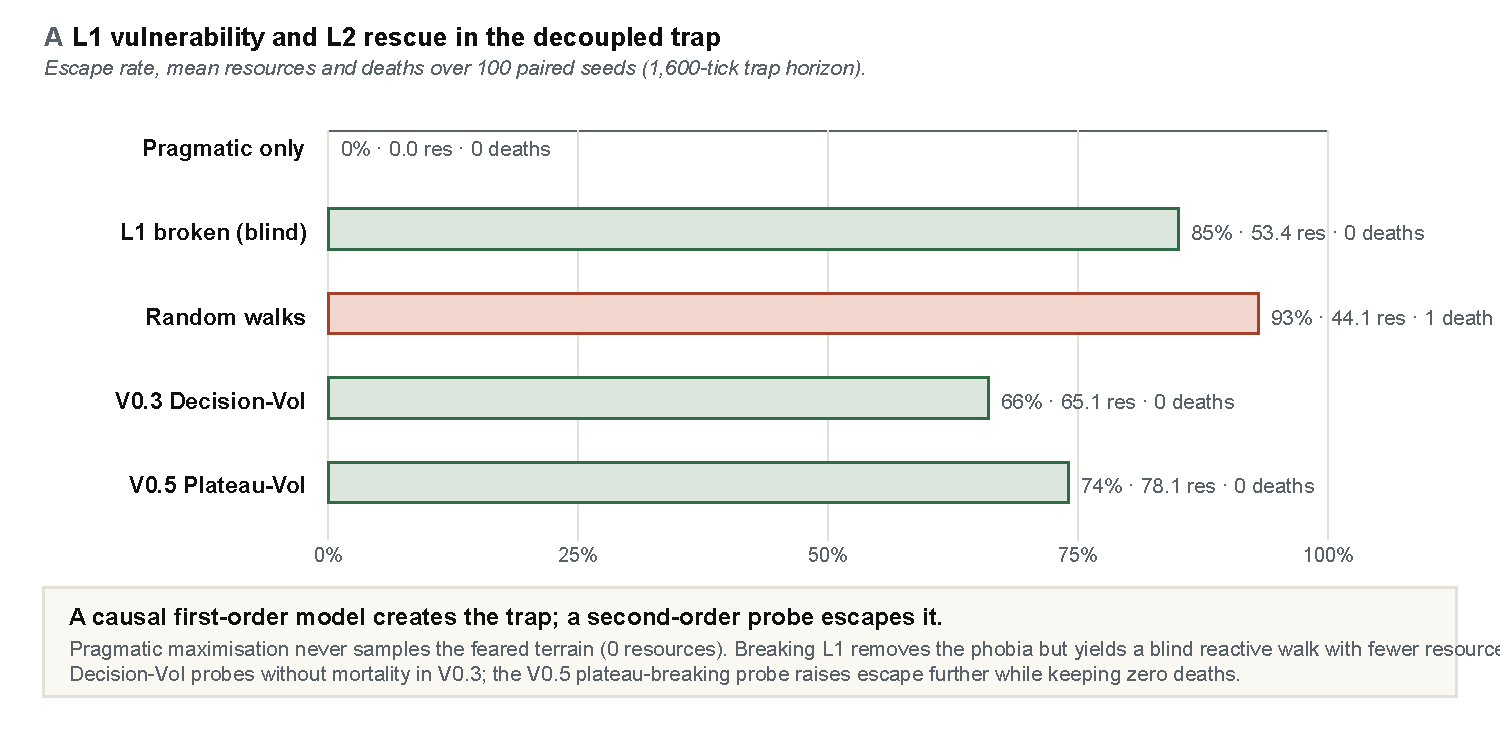
\includegraphics[width=\linewidth]{figures/fig3_epistemic_trap_escape}
\caption{The decoupled epistemic trap. Pragmatic maximisation never samples the feared terrain and starves. Breaking L1 removes the phobia but yields a blind reactive walk with fewer resources. Random exploration escapes more but at lower resources and with a death. Decision-VoI escapes without mortality; the V0.5 plateau probe raises escape and resources while keeping zero deaths.}
\label{fig:trap}
\end{figure}

\section{Precision predictive coding, the attention schema, and the trilemma}

\subsection{PP-1: precision-weighted filtering}

V0.4 introduces a precision-weighted filter. Each channel has a precision weight $\pi_i$; the posterior gain is a precision ratio, in the spirit of the Kalman gain \citep{kalman1960new}:
\begin{equation}
K_i = \frac{\pi_i}{\pi_i + \sigma_i^2\lambda},
\qquad
\hat{y}_i \leftarrow \hat{y}_i + K_i\,(y_i - \hat{y}_i).
\end{equation}
A single-channel outlier collapses the precision of that channel for one tick, absorbing a transient illusion. Sustained cross-channel disagreement instead erodes the prior precision. The intended consequence is a short, bounded influence of a spurious pulse.

\subsection{AST-1: a schema over internal precision}

AST-1 adds a five-window model of the agent's own precision weights. The schema estimates whether the agent is currently in a high-prior or high-sensor mode, and releases suppression when the disagreement that justified it has ended. The behavioural signature is post-glitch recovery: after a transient sensor anomaly, a filter without the schema remains stuck in a distrustful mode; with the schema, the agent returns to its normal gain.

In V0.4, schema-on versus schema-off recovery is $\mathbf{0.237}$ vs $\mathbf{0.181}$ (40 paired glitch runs, $dz=1.13$, $p<0.001$). The effect is smaller in V0.5 because selective gating already avoids most normal-operation suppression, leaving less perseverance for the schema to release.

\subsection{The illusion--tracking--diagnostic trilemma}

\begin{table}[t]
\centering
\small
\caption{The illusion--tracking--diagnostic trilemma at 100 paired seeds. V0.5 absorption is the 20-seed pilot because the 100-seed harness still runs the legacy probe.}
\label{tab:trilemma}
\begin{tabular}{lcccc}
\toprule
Version & PP-1 absorption & Stationary MAE & Attribution macro-F1 & Trap escape \\
\midrule
V0.3 & $\approx 0.00$ & \textbf{1.68} & \textbf{0.604} & 66/100 \\
V0.4 & \textbf{0.830 [0.811, 0.848]} & 2.74 & 0.515 & 65/100 \\
V0.5 & 0.79 (pilot) & 2.04 & 0.577 & \textbf{74/100} \\
\bottomrule
\end{tabular}
\end{table}

The three targets cannot be maximised at once (Table~\ref{tab:trilemma}, Figure~\ref{fig:trilemma}). Absorbing the illusion requires trusting the prior, which is the same gain that slows tracking. In V0.4 the cost is explicit: absorption rises from zero to 0.830 while stationary MAE rises from 1.68 to 2.74 and attribution macro-F1 falls from 0.604 to 0.515. V0.5's selective gating recovers part of the tracking cost (MAE 2.04) and part of the diagnostic cost (F1 0.577), but it does not reach V0.3's accuracy, and its absorption is measured only in the 20-seed pilot.

The trilemma is the paper's central negative result. It is a \emph{frontier}, not a failure of implementation: each point is the best achievable given the same precision gain, and moving along the frontier changes which capability is sacrificed.

At the full protocol V0.5 also reaches rolling BSS $\mathbf{0.027\ [0.025,0.028]}$ and latent-failure AUROC $\mathbf{0.785\ [0.773,0.797]}$, and the learned world model beats the neutral ablation by $\mathbf{+4.72\ [0.77,8.68]}$ resources ($dz=0.22$, $p=0.027$). The world-model advantage lost in V0.4 is therefore recovered, but at a tracking and diagnostic cost (Figure~\ref{fig:progression}).

\subsection{The Goodhart check}

A local metacognitive score can improve while system outcomes do not. We therefore test whether lower meta-Brier loss \citep{brier1950verification} predicts more resources across seeds. The correlation is $\mathbf{r=0.313}$, and the induced resource change is $\mathbf{+0.57\ [-3.47,4.73]}$ (n.s.). Local calibration and system-level success are related but not substitutable. An indicator programme that optimises the local score without checking the system outcome would report progress that the agent does not experience as improved survival.

\begin{figure}[t]
\centering
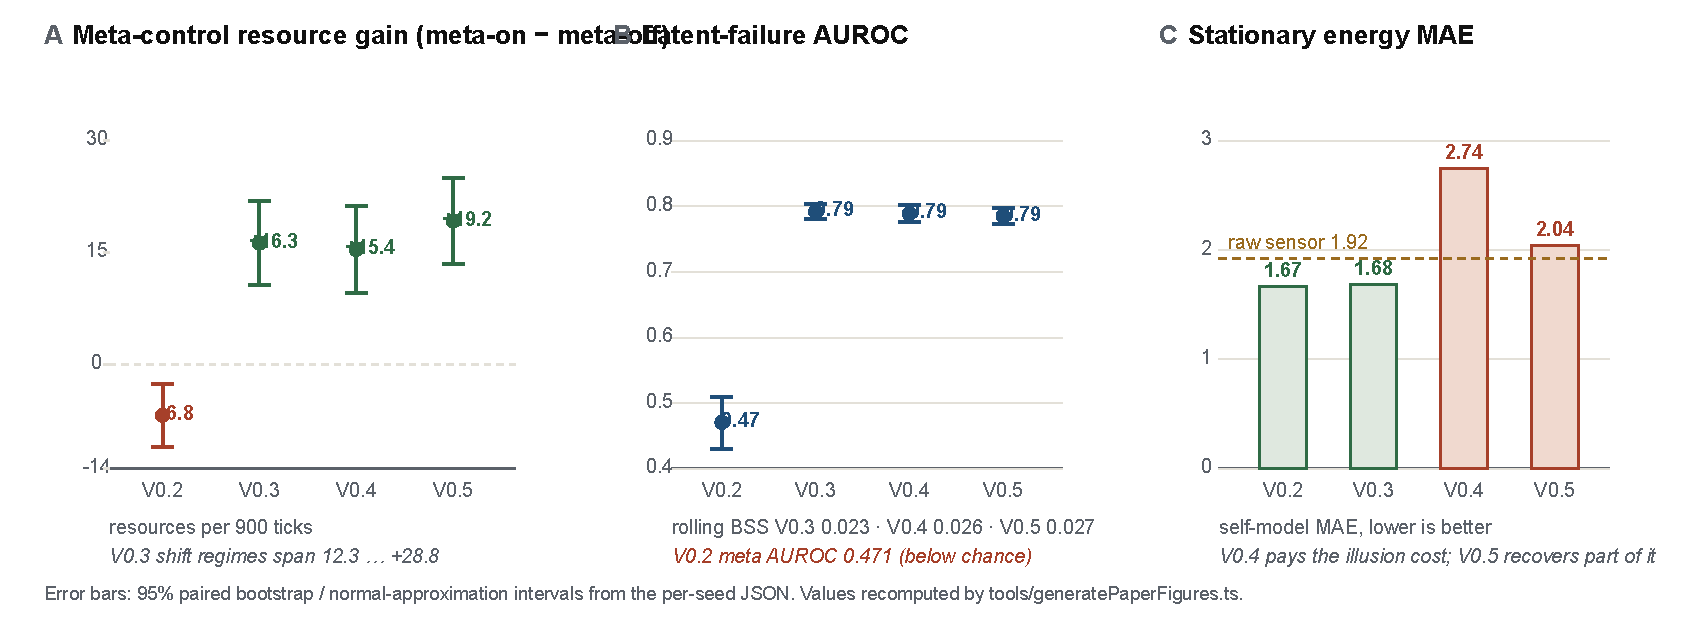
\includegraphics[width=\linewidth]{figures/fig2_cross_version_progression}
\caption{Cross-version progression at 100 paired seeds. (A) Meta-control resource gain (meta-on $-$ meta-off) with 95\% intervals: V0.2 is negative, V0.3--V0.5 positive; the V0.3 shift regimes span $+12.34$ to $+28.82$. (B) Latent-failure AUROC: below chance in V0.2, stable near 0.79 from V0.3. (C) Stationary energy MAE against the raw interoceptive reference (1.92); V0.4 pays the illusion cost, V0.5 recovers part of it.}
\label{fig:progression}
\end{figure}

\begin{figure}[t]
\centering
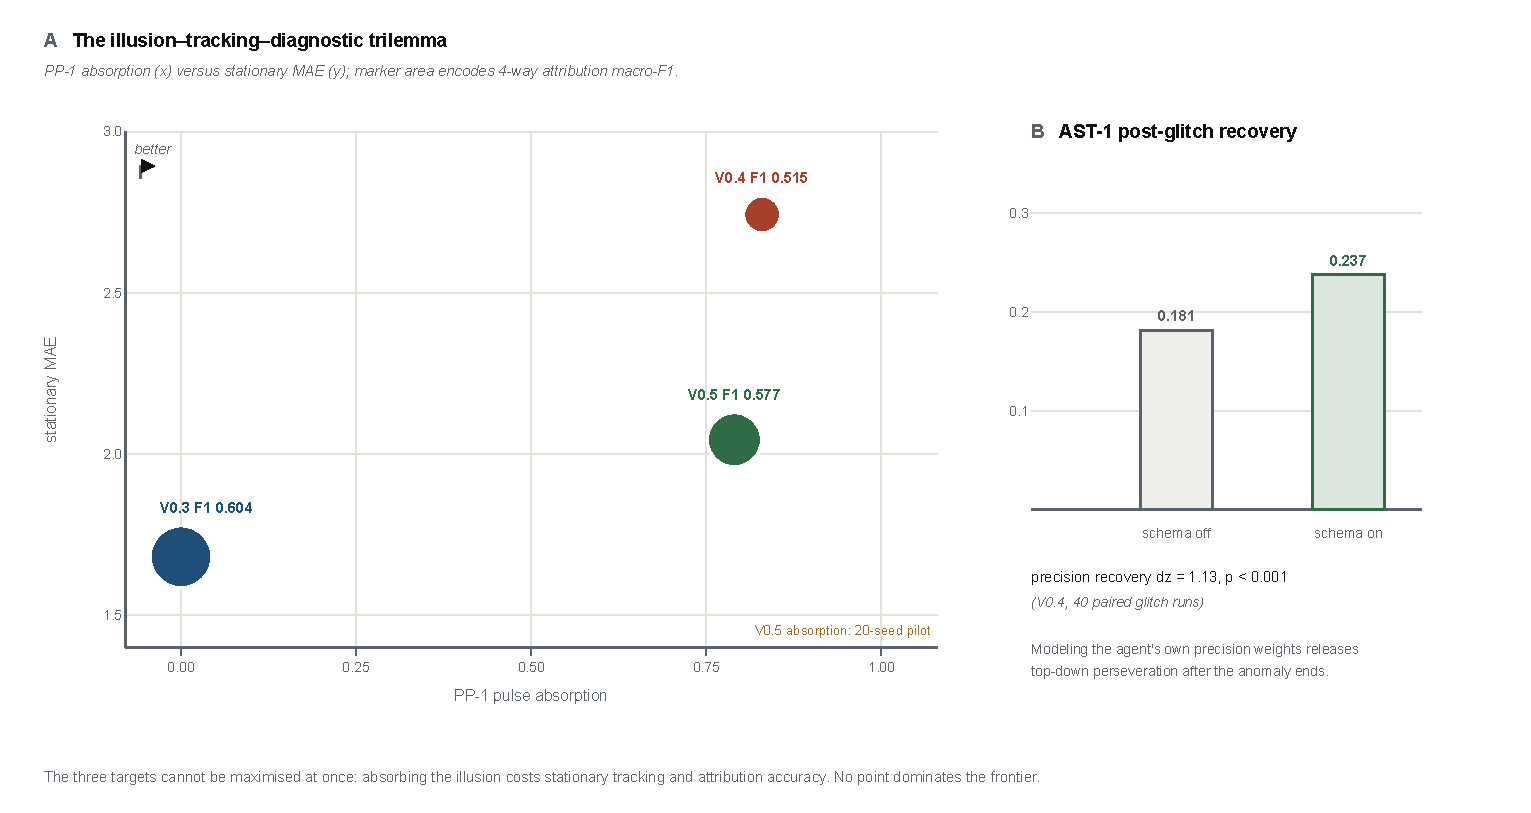
\includegraphics[width=\linewidth]{figures/fig4_trilemma_pareto}
\caption{The illusion--tracking--diagnostic trilemma. PP-1 absorption is plotted against stationary MAE, with marker area encoding four-way attribution macro-F1. V0.4 buys absorption with tracking and attribution; V0.5 recovers part of both without dominating V0.3. Inset: AST-1 post-glitch recovery, schema on versus off ($dz=1.13$, $p<0.001$, 40 paired glitch runs).}
\label{fig:trilemma}
\end{figure}

\section{A unified architecture under adversarial control (V0.6)}

The first five generations ask what a self-model buys. V0.6 asks whether the integrated,
self-referential mechanisms are \emph{causally necessary} for a set of cognitive capabilities, and
whether those capabilities survive comparison with matched-compute alternatives. It is a
different experiment, not a sixth survival iteration.

\paragraph{Architecture.}
Four specialist modules---world, somatic, meta-attribution and epistemic---each return an
independent proposal (preferred action, five utilities, salience, confidence, goal and evidence).
Salience is computed on the deviation from the shared pragmatic baseline, so a module that merely
restates the baseline cannot capture the workspace. A capacity-limited workspace ignites one
coalition, with weight $1-0.14(n-1)$ for the winner and $0.14$ for the others, and broadcasts an
action bias, a precision plan and per-module learning gains back to all four modules. A recurrent
sheet settles bottom-up evidence and the top-down prior over $K=3$ passes and modulates the V0.5
precision gain rather than replacing it. A higher-order monitor estimates reliability, calibrates a
shadow head on off-policy probes, attributes discrepancies to self, energy, fatigue or shared
causes, and projects the integrated state into a three-axis quality space. An attention schema
models its own precision allocation and emits a recovery signal. A four-step rollout simulates
future physical state, future belief uncertainty, future reliability and future workspace mode; the
epistemic option value is the value of the decisions that a resolved uncertainty would unlock.

\begin{table}[h]
\centering
\caption{V0.6 indicator experiments at 100 paired seeds. The contrast is intact minus the named
ablation or control; intervals are 95\% bootstrap CIs.}
\label{tab:v06}
\begin{tabular}{llll}
\toprule
Experiment & Intact & Ablation / control & Contrast \\
\midrule
Ambiguous settling & absorption 0.814 & No-RPT 0.290 & $+0.524\ [0.482,0.567]$, $d_z=2.38$ \\
Compound conflict & thrash 0.051 & No bottleneck 0.356 & $-0.304\ [-0.344,-0.266]$, $d_z=-1.53$ \\
Goal coherence & 0.91 & 0.68 & $+0.23\ [0.21,0.24]$, $d_z=2.57$ \\
Post-conflict recovery & 19 ticks & No-AST 256 & $-236.9\ [-245.3,-226.6]$ \\
Sensor attribution & macro-F1 0.502 & No-HOT 0.000 & routing 0.774 [0.747, 0.799] vs 1.00 \\
Epistemic fork & 94\% probe / 84\% solved & No-AE 1\% / 1\% & $+0.83\ [0.75,0.90]$, $d_z=2.20$ \\
Contingency reversal & 2.1-tick detection & No-HOT 400 (never) & $+397.9\ [394.2,397.7]$ \\
\bottomrule
\end{tabular}
\end{table}

The double dissociation is the central result. Capacity competition is necessary for policy
coherence under simultaneous demands; broadcast is necessary for binding even when the winner is
held fixed; the higher-order monitor is necessary for attribution, selective plasticity routing and
first-order accuracy under sensor corruption; the attention schema is necessary for recovery; and
cognitive self-simulation is necessary for paying the immediate cost of a diagnostic probe, and
recurrent settling is necessary for single-tick absorption. A physical-only MPC planner with the
same horizon and action space probes in only 2\% of runs and solves 1\%, which isolates the cognitive
state prediction rather than the planning horizon.

\paragraph{What failed.}
Three results constrain the interpretation. First, the fork now solves 84\% of runs but remains
one point below the 85\% target. Second, reliability calibration still fails: shadow AUROC is 0.46
self, 0.59 energy, 0.43 fatigue and 0.58 shared, all below 0.75. Third, attribution is
class-imbalanced: 0.502 macro-F1 with shared recall 0.39, even though physical recall is 0.90.

Generalization is mixed. With zero re-tuning, the architecture wins the fork (84\% vs 4\%
reactive / 1\% MPC / 73\% flat / 31\% feedforward) and conflict coherence (0.915 vs 0.666
flat / 0.831 reactive), but flat and reactive controls out-forage it in standard shift, conflict
and the compound suite (32.7 vs 47.5 in Gen3). The architecture is a stronger instrument, not a
better forager.

\section{Discussion, limitations, and reproducibility}

\paragraph{Why negative results matter.}
The V0.1 audit, the V0.2 sign error, the V0.4 tracking cost and the V0.5 non-Pareto outcome are not appendix material; they are the evidence that the indicator properties are doing work. A benchmark that reported only the V0.3 breakthrough would invite Goodharting: the next architecture could maximise the reported indicator while degrading the system it is supposed to explain. Reporting the frontier makes that trade visible.

\paragraph{Functional versus phenomenal.}
$M_1$ and $M_2$ are predictors and controllers. ``Self-model'', ``meta-model'', ``attention schema'' and ``strange loop'' name computational objects with measurable behaviour. The lab does not claim that the agent is conscious, sentient or has subjective experience, and no metric is labelled a consciousness score. The contribution to the science of consciousness is methodological: a transparent testbed in which indicator properties can be operationalised, ablated and priced.

\paragraph{Limitations.}
The world is small and discrete; the agent is non-neural; the horizon is 900 ticks (1{,}600 in traps, 1{,}200 in the V0.6 fork); the reported generations are six architectures, not a search over architectures. The 20-seed PP-1 pilot for V0.5 and the 40-run AST estimate in V0.4 are smaller samples than the main protocol and are flagged as such. The 100-seed harness does not re-estimate absorption for V0.5. The V0.6 option-value term is an explicit architectural prior; the epistemic-fork result isolates its necessity within this architecture, not the impossibility of physical planners. Generalisation to neural or open-ended systems is not claimed.

\paragraph{Future work.}
Four questions follow directly from this record.
\begin{enumerate}
  \item A preregistered sweep of the precision-decay and AST-1 recovery parameters would map a continuous Pareto frontier instead of the five architectural points sampled here.
  \item Decision-VoI and plateau preparation should be stress-tested under multi-step lookahead, delayed or ambiguous effort feedback, and environments where rough terrain is occasionally genuinely lethal.
  \item Temporal attribution should be separated into calibration and discrimination under explicitly held-out shift schedules, particularly for the physical-versus-fatigue confusion.
  \item The observable-outcome interface used by the learning calls in V0.2--V0.5 should be extended to every evaluation reachable from agent code, so the no-ground-truth guarantee is auditable end to end by the type system rather than by code review alone.
\end{enumerate}

\paragraph{Reproducibility.}
Every run is seeded and deterministic. The repository preserves all six engines, their tests, dashboards and reports:
\begin{verbatim}
npm run validate        # V0.1, 100 seeds
npm run validate:v02    # V0.2, 100 seeds
npm run validate:v03    # V0.3, 100 seeds
npm run validate:v04    # V0.4, 100 seeds
npm run validate:v05    # V0.5, 100 seeds (SEEDS=100 default)
npm run validate:v06    # V0.6, 100 seeds, 87 conditions (8,700 episodes)
npm run paper:figures   # regenerate paper/figures/*.svg
npm run typecheck && npm test && npm run build
\end{verbatim}
Raw per-run JSON is in \texttt{research/}; aggregate reports are in \texttt{docs/}. The UI exposes the same numbers with plain-English and statistical layers. The 28{,}100 total is the main protocol; adding the 800 V0.1 corruption observations gives 28{,}900 logged runs.

\paragraph{Data and code availability.}
The interactive laboratory is at \url{https://strangeloops.pages.dev}. The complete source, the six engines, their tests, the validation harnesses, the per-run JSON artifacts in \texttt{research/}, the reports in \texttt{docs/}, and the figure generator are maintained as one repository; an archived snapshot is available from the author on request. Every figure and statistic in this manuscript can be regenerated from the JSON with \texttt{npm run paper:figures} and the validation commands listed above.

\paragraph{Use of AI tools.}
Generative AI tools were used in this work as follows. (i) An agentic coding environment (OpenCode, 2026; model identifiers and dates are retained in the project transcript) drafted and edited TypeScript for the engines, validation harnesses, UI and figure generator, and ran the validators. (ii) The same environment drafted and edited prose, tables and the \LaTeX/Markdown sources, and assisted in checking reported values against the JSON artifacts. (iii) All figures are produced by deterministic TypeScript from the JSON; no generative image model produced, altered or enhanced any figure or datum. The author specified the research question, design and acceptance criteria, reviewed every change, verified the references against their published sources, and takes full responsibility for all content. Every reported number was regenerated from the checked-in JSON; the 73-test suite and the type check pass on the archived code.

\paragraph{Declarations.}
\textit{Funding:} none. \textit{Competing interests:} none. \textit{Author contributions:} Anand Jayakumar conceived the study, designed the architectures and protocols, implemented and reviewed the code, ran and audited the validations, and wrote the manuscript. \textit{Ethics:} no human participants or animals were involved, and no personal data were processed.

\bibliography{references}

\end{document}
